\def\scl{0.6}%scaling factor of the picture
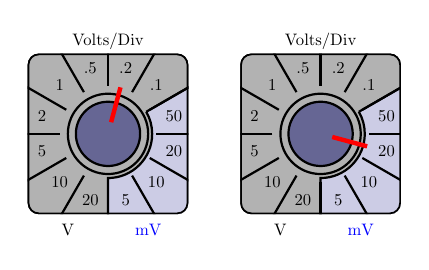
\begin{tikzpicture}[
  scale=\scl,
  controlpanels/.style={yellow!30!brown!20!,rounded corners,draw=black,thick},
  screen/.style={green!50!black!60!,draw=black,thick},
  trace/.style={green!60!yellow!40!, ultra thick},
  smallbutton/.style={white,draw=black, thick},
  axes/.style={thick}]
  % \fill[green!30!blue!30!,rounded corners,draw=black,thick](0,0)
  %   rectangle (27.75,13.25);
  % \fill[fill=black!40!,draw=black,thick,rounded corners](0.25,0.25)
  %   rectangle (27.5,13.00);

% Lower right panel
  % \fill[controlpanels] (13.7,0.5) rectangle (27.1,6.2);
  % %Channels
  % % CH I
  % \draw[thick] (14.8,1.5) circle (0.7cm);
  % \fill[gray,draw=black,thick] (14.8,1.5) circle (0.5cm);
  % \fill[white,draw=black,thick] (14.8,1.5) circle (0.3cm);
  % \node[scale={1.5*\scl}] at (14.8,2.5) {CH I};
  % \draw[thick] (16.2,1.5) circle (0.4cm);
  % \fill[black!60!] (16.2,1.5) circle (0.3cm);
  % \draw[thick] (16.6,1.5) --(17,1.5)--(17,1.0);
  % \draw[thick] (16.7,1.0)--(17.3,1.0);
  % \draw[thick] (16.8,0.85)--(17.2,0.85);
  % \draw[thick] (16.9,0.70)--(17.1,0.70);
  % \draw[thick] (26.0,1.5) circle (0.7cm);
  % % CH II
  % \fill[gray,draw=black,thick] (26,1.5) circle (0.5cm);
  % \fill[white,draw=black,thick] (26,1.5) circle (0.3cm);
  % \node[scale={1.5*\scl}] at (26,2.5) {CH II};
  % \draw[thick] (24.6,1.5) circle (0.4cm);
  % \fill[black!60!] (24.6,1.5) circle (0.3cm);
  % \draw[thick] (24.2,1.5) --(23.7,1.5)--(23.7,1.0);
  % \draw[thick] (23.4,1.0)--(24.0,1.0);
  % \draw[thick] (23.5,0.85)--(23.9,0.85);
  % \draw[thick] (23.6,0.70)--(23.8,0.70);
  % \draw[thick] (26.0,1.5) circle (0.7cm);
  % Y-pos
  % \fill[smallbutton] (14.8,4.9) circle (0.3cm);
  % \node[scale={\scl}] at (14.8,5.5) {Y-pos I};
  % \fill[smallbutton] (26.0,4.9) circle (0.3cm);
  % \node[scale={\scl}] at (26.0,5.5) {Y-pos II};
  % Volt/div the foreach loop draws the two buttons
  \foreach \i / \b in {18/75,22.5/345}{
  %Second parameter of the loop is the angle of the index mark 
  \begin{scope}[xshift=\i cm,yshift=3.8cm,scale=0.85]
    \node[scale=\scl] at (0,2.3) {Volts/Div};
    \node[scale=\scl,black] at (-1,-2.4) {V};
    \node[scale=\scl,blue]  at (1,-2.4) {mV};
    \clip[rounded corners] (-2,-2) rectangle (2,2);
    \fill[black!30!,rounded corners,draw=black,thick] (-2,-2)
      rectangle (2,2);
    \fill[blue!50!black!20!,draw=black,thick]
      (30:1.1)--(30:3)--(3,-3)--(-90:3)--(-90:1.1) arc (-90:30:1.1);
    \draw[very thick,rounded corners](-2,-2) rectangle (2,2);
    \draw[thick] (0,0) circle (1.0);
    \foreach \i in {0,30,...,330}
      \draw[thick] (\i:1.2)--(\i:2.5);
    \foreach \i/\j in {15/50,45/.1,75/.2,105/.5,135/1,165/2,195/5,225/10,
      255/20,285/5,315/10,345/20} \node[scale=\scl,black] at (\i:1.7) {\j};
    \fill[blue!30!black!60!,draw=black,thick] (0,0) circle (0.8cm);
    % Here you set the right Volts/Div button
    \draw[ultra thick,red] (\b:0.3)--(\b:1.2);
  \end{scope}}
  \end{tikzpicture}
